\documentclass{mcmthesis}
\mcmsetup{CTeX = false, 
        tcn =57566, problem = B,
        sheet = true, titleinsheet = true, keywordsinsheet = true,
        titlepage = false, abstract = true}
\usepackage{palatino}
\usepackage{array}
\bibliographystyle{apalike}
\title{An optimized design of the area following the toll barrier }

\begin{document}

	
	
\begin{abstract}
	
In order to determine the optimal area following the toll barrier, this paper proposes a function model for the turnpike authority in favor of the promotion of the toll station.

First, after seeking examples of toll stations in common use and analyzing the complicated situations, we enumerate the important elements which will quantify the performance of the station design. The performance is mainly constituted by throughput, accident rate and cost. Their weights are determined by principal component analysis. 

Next, we apply Nagel-Schreckenberg (NS) model and then develop a function model to simulate the process for vehicles to pull out and every decision made by observing the surroundings. Meanwhile we can model the accident probability as well. In which way the quantity of vehicles via the toll station in unit time is obtained. And the cost is defined by the area the station takes and the number and proportions of tollbooths. 

Then, according to this generalized adaptive model, we can adjust some parameters to reach a bigger throughput. And we recalculate accident rate and cost. By means of adjustments and experiments on MATLAB, a better solution with obvious advantage is designed. Its size, shape and merging pattern are detailed in our report.

Finally, with different parameters set, the condition of heavy traffic or light traffic is established, in which we compare the performance of our design with the common ones. The situation where more autonomous vehicles are added or the proportions of tollbooths are changed can also be tested in this model. The result turns out that our solution is an optimized design.

   
  
  
  
\begin{keywords}
 Nagel-Schreckenberg (NS) model;
\end{keywords}
\end{abstract}

\maketitle
\tableofcontents
\clearpage








\section{A letter to the New Jersey Turnpike Authority}


New Jersey Turnpike Authority,

Our team has proposed an optimized toll station design allowing the increase of throughput and the decrease of cost and accident rate. And a new mathematical model is built in order to help evaluate the performances of designs. 

More specifically, the performance model is developed after taking all important elements related to this problem into consideration, like number of lanes and tollbooths, proportions of tollbooths, varieties of vehicles, change of flows, every decision made by drivers to turn right or left and traffic conditions. 



\section{Introduction}

\subsection{Statement of the problem}

  The design of toll station is undoubtedly a kind of art as it is hard to find a balance among safety, capacity and cost facing different situations. But it also acts as an essential part in the high-way traffic system. As a promotion of toll station is in demand, we apply mathematical methods and function models for optimize our design, striving to increase the throughput, decrease the cost and accident rate.


\begin{itemize}

\item 
\end{itemize}







\begin{Theorem} \label{thm:latex}

\end{Theorem}

\begin{Lemma} \label{thm:tex}

\end{Lemma}

\begin{proof}
The proof of theorem.
\end{proof}

\subsection{Assumptions}

\begin{itemize}
	\item All the vehicles leave the tollbooths with a given speed.
	\item There is a critical flow $F_c$, when the total flow  $F_t>F_c$, the vehicles begin to queue up before the toll station.
	\item The proportions of different types of vehicles are invariable along the time.
	\item In light traffic, the tollbooths the vehicles arrive are random.
	\item We apply Nagel-Schreckenberg (NS) model here.
\end{itemize}



Here we list the elements that will influence the throughput of our toll station:

\begin{tabular}{|m{7cm}<{\centering}|p{7cm}<{\centering}|}
	\hline
	Notations & Meanings \\
	\hline
	 $L$ &  Number of lanes \\
	\hline
	 $B$ &  Number of tollbooths\\
	 \hline
     $F_t$ & 	 Total flow\\
     \hline
     $F_c$ & Critical flow (the maximum of the total flow)\\
     \hline
     $P_l$,  $P_m$, $P_s$ & Probability of large-scale automobiles, midium-sized vehicles and compact cars\\
     \hline
    $C$ & Cell size (in the model Nagel-Schreckenberg (NS) that we will use)\\
    \hline
     
\end{tabular}

\begin{itemize}
\item
\item
\item
\item
\end{itemize}



\section{Analysis of the Problem}
\begin{figure}[htbp]
\small
\centering
\caption{Toll station \cite{note}} \label{fig:Ts}
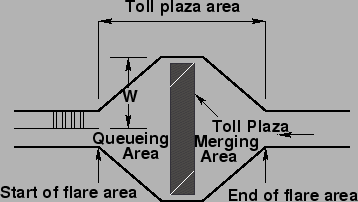
\includegraphics{img3.png}
\end{figure}


\section{Calculating and Simplifying the Model  }


\section{The Model Results}


\section{Validating the Model}


\section{Conclusions}

\section{A Summary}


\section{Evaluate of the Mode}

\section{Strengths and weaknesses}


\subsection{Strengths}
\begin{itemize}
\item \textbf{Applies widely}\\

\item \textbf{Improve the quality of the airport service}\\

\item \textbf{}\\
\end{itemize}


\begin{appendices}

\section{First appendix}


Here are simulation programmes we used in our model as follow.\\

\textbf{\textcolor[rgb]{0.98,0.00,0.00}{Input matlab source:}}
\lstinputlisting[language=Matlab]{./code/matlab1.m}

\section{Second appendix}

some more text \textcolor[rgb]{0.98,0.00,0.00}{\textbf{Input C++ source:}}
\lstinputlisting[language=C++]{./code/sudoku.cpp}

\end{appendices}

	\nocite{*}

\bibliography{math}

	
\end{document}

